\Large\textbf{}\\
\Large\textbf{Use Case 1 - Creazione nuovo layout} \\
\vspace{0.5cm}
%\begin{figure}[h]
%  \centering
%  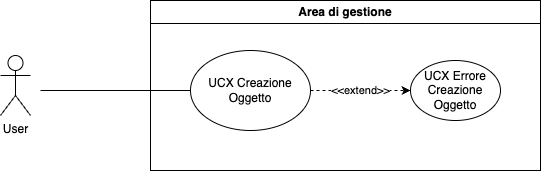
\includegraphics[width=0.8\textwidth]{UseCasesImages/ObjCr.png}
%\end{figure}
\large\textbf{} \\
\textbf{Attori:} User\\
\textbf{Pre-condizione:} Avvio dell'applicazione da parte dell'utente\\
\textbf{Post-condizione: } Creazione del layout magazzino\\
\textbf{Scenario Principale:}  All'utente viene richiesto se caricare un layout esistente o se creare un nuovo layout.\\
\vspace{0.5cm}

\Large\textbf{}\\
\Large\textbf{Use Case 1.1 - Creazione Nuovo magazzino} \\
\vspace{0.5cm}
%\begin{figure}[h]
%  \centering
%  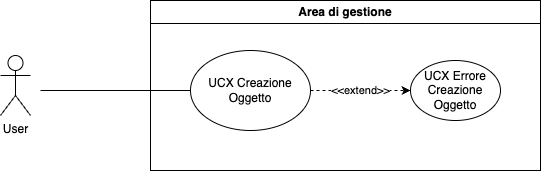
\includegraphics[width=0.8\textwidth]{UseCasesImages/ObjCr.png}
%\end{figure}
\large\textbf{} \\
\textbf{Attori:} User\\
\textbf{Pre-condizione:} E' stata selezionata la modalità: "Creazione manuale magazzino" \\
\textbf{Post-condizione: } Nuovo layout magazzino creato correttamente\\
\textbf{Scenario Principale:}  L'utente viene invitato ad inserire le dimensioni del magazzino in modo da poterne creare il layout di base. In particolare dovrà inserire:
    \begin{itemize}
        \item Ampiezza del magazzino
        \item Profondità del magazzino 
        \item Altezza del magazzino 
    \end{itemize}
\textbf{Estensioni: } UC1.1.1 - Errore Creazione nuovo magazzino\\
\vspace{0.5cm}

\Large\textbf{}\\
\Large\textbf{Use Case 1.1.1 - Errore Creazione nuovo magazzino} \\
\vspace{0.5cm}
\large\textbf{} \\
\textbf{Attori:} User\\
\textbf{Pre-condizione:} L'utente ha appena inserito le tre dimensioni per creare il layout del nuovo magazzino \\
\textbf{Post-condizione: } Visualizzazione messaggio di errore\\
\textbf{Scenario Principale:}  Il sistema, dopo aver ricevuto in input le dimensioni per creare il nuovo magazzino, verifica e segnala un errore sulle stesse.\\ 
\vspace{0.5cm}

\Large\textbf{}\\
\Large\textbf{Use Case 1.2 Importazione layout magazzino} \\
\vspace{0.5cm}
%\begin{figure}[h]
%  \centering
%  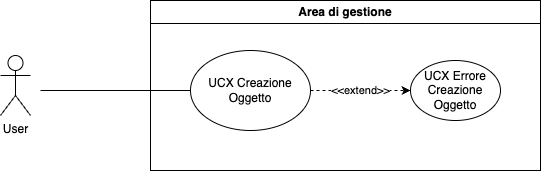
\includegraphics[width=0.8\textwidth]{UseCasesImages/ObjCr.png}
%\end{figure}
\large\textbf{} \\
\textbf{Attori:} User\\
\textbf{Pre-condizione:} E' stato selezionata la modalità: "Importazione layout magazzino" \\
\textbf{Post-condizione: } Importazione Layout Magazzino\\
\textbf{Scenario Principale:}  L'utente viene invitato a selezionare un file esistente da importare. Verrà utilizzato per caricare il layout di un magazzino già creato e salvato.\\
\textbf{Estensioni: } UC1.2.1 - Errore importazione Layout\\
\vspace{0.5cm}

\Large\textbf{}\\
\Large\textbf{Use Case 1.2.1 Errore importazione layout} \\
\vspace{0.5cm}
\large\textbf{} \\
\textbf{Attori:} User\\
\textbf{Pre-condizione:} E' stato selezionata il file che verrà utilizzato per caricare il layout del magazzino \\
\textbf{Post-condizione: } Visualizzazione messaggio di errore\\
\textbf{Scenario Principale:}  Il sistema, dopo aver ricevuto in input il file attraverso cui caricare il layout magazzino, segnala un errore in fase di caricamento del layout esistente.\\
\vspace{0.5cm}

\Large\textbf{}\\
\Large\textbf{Use Case 2 - Modifica layout magazzino} \\
\vspace{0.5cm}
%\begin{figure}[h]
%  \centering
%  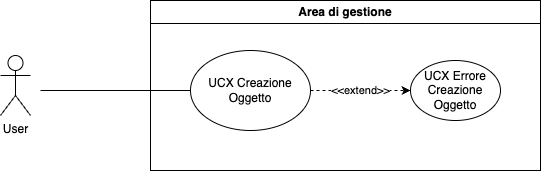
\includegraphics[width=0.8\textwidth]{UseCasesImages/ObjCr.png}
%\end{figure}
\large\textbf{} \\
\textbf{Attori:} User\\
\textbf{Pre-condizione:} L'utente seleziona il comando "Modifica layout magazzino"\\
\textbf{Post-condizione: } Modifica apportata correttamente\\
\textbf{Scenario Principale:}  L'utente avrà la possibilità di modificare la struttura del magazzino in due modalità: 
\begin{itemize}
    \item Trascinare le freccie presenti nei vari lati tridimensionali del per aumentare o ridurne le dimensioni
    \item Inserire le nuove dimensioni nell'apposito campo di "modifica assistita"
\end{itemize}
\textbf{Estensioni: } UC2.1 - Errore modifica layout\\
\vspace{0.5cm}

\Large\textbf{}\\
\Large\textbf{Use Case 2.1 - Errore modifica layout} \\
\vspace{0.5cm}
\large\textbf{} \\
\textbf{Attori:} User\\
\textbf{Pre-condizione:} Sono state inserite, attraverso il form di "modifica assistita" le nuove dimensioni del magazzino \\
\textbf{Post-condizione: } Visualizzazione messaggio di errore\\
\textbf{Scenario Principale:}  Il sistema, dopo aver ricevuto in input le nuove dimensioni del magazzino, segnala un errore in fase di adeguamento alle nuove dimensioni.\\
\vspace{0.5cm}

\Large\textbf{}\\
\Large\textbf{Use Case 3 - Salvataggio layout} \\
\vspace{0.5cm}
%\begin{figure}[h]
%  \centering
%  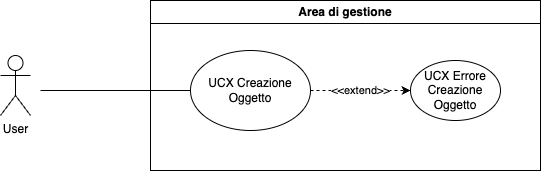
\includegraphics[width=0.8\textwidth]{UseCasesImages/ObjCr.png}
%\end{figure}
\large\textbf{} \\
\textbf{Attori:} User\\
\textbf{Pre-condizione:} L'utente seleziona il comando "Salva layout"\\
\textbf{Post-condizione: } Il layout in corso viene correttamente salvato su appposito file \\
\textbf{Scenario Principale:}  L'utente avrà la possibilità di indicare il percorso e il nome del nuovo file in cui verrà salvato il layout corrente \\ 
\textbf{Estensioni: } UC3.1 - Errore salvataggio layout\\
\vspace{0.5cm}

\Large\textbf{}\\
\Large\textbf{Use Case 3.1 - Errore salvataggio layout} \\
\vspace{0.5cm}
\large\textbf{} \\
\textbf{Attori:} User\\
\textbf{Pre-condizione:} L'utente ha indicato la posizione e il nome da assegnare al file sul quale verrà salvato il layout corrente \\
\textbf{Post-condizione: } Visualizzazione messaggio di errore\\
\textbf{Scenario Principale:}  Il sistema, dopo aver ricevuto in input i dati richiesti, segnala un errore in fase di salvataggio del layout su file.\\
\vspace{0.5cm}

\Large\textbf{}\\
\Large\textbf{Use Case 4 - Creazione scaffalatura} \\
\vspace{0.5cm}
%\begin{figure}[h]
%  \centering
%  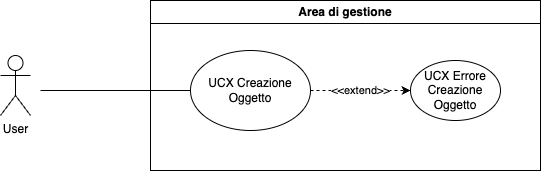
\includegraphics[width=0.8\textwidth]{UseCasesImages/ObjCr.png}
%\end{figure}
\large\textbf{} \\
\textbf{Attori:} User\\
\textbf{Pre-condizione:} L'utente selezione il comando "Crea nuova scaffalatura" \\
\textbf{Post-condizione: } Creazione corretta della scaffalatura\\
\textbf{Scenario Principale:}  L'utente, attraverso il muose, può selezionare il punto di creazione della scaffalatura e da esso estenderla nei due lati possibili, altezza e lunghezza. \\
\vspace{0.5cm}

\Large\textbf{}\\
\Large\textbf{Use Case 5 - Selezione scaffalatura} \\
\vspace{0.5cm}
%\begin{figure}[h]
%  \centering
%  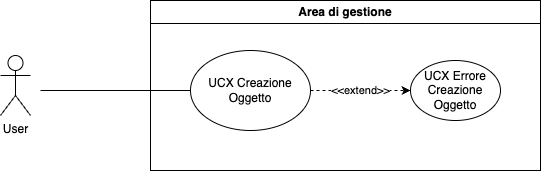
\includegraphics[width=0.8\textwidth]{UseCasesImages/ObjCr.png}
%\end{figure}
\large\textbf{} \\
\textbf{Attori:} User\\
\textbf{Pre-condizione:} L'utente ha creato correttamente il layout \\
\textbf{Post-condizione: } Visualizzazione dati scaffalatura e evidenziazione a video\\
\textbf{Scenario Principale:}  L'utente preme il tasto sinistro del mouse sopra la struttura di una scaffalatura\\
\vspace{0.5cm}

\Large\textbf{}\\
\Large\textbf{Use Case 6 - Spostamento scaffalatura} \\
\vspace{0.5cm}
%\begin{figure}[h]
%  \centering
%  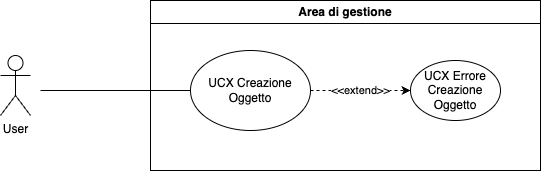
\includegraphics[width=0.8\textwidth]{UseCasesImages/ObjCr.png}
%\end{figure}
\large\textbf{} \\
\textbf{Attori:} User\\
\textbf{Pre-condizione:} L'utente seleziona il comando "Spostamento scaffalatura" \\
\textbf{Post-condizione: } Scaffallatura correttamente spostata \\
\textbf{Scenario Principale:}  L'utente selezione la scaffalatura da spostare e la trascina verso il nuovo spazio di posizionamento.\\
\vspace{0.5cm}

\Large\textbf{}\\
\Large\textbf{Use Case 7 - Modifica scaffalatura} \\
\vspace{0.5cm}
%\begin{figure}[h]
%  \centering
%  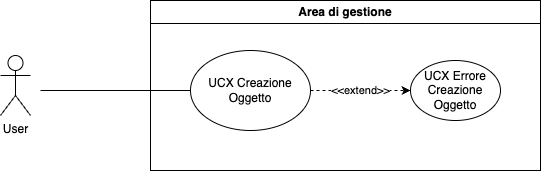
\includegraphics[width=0.8\textwidth]{UseCasesImages/ObjCr.png}
%\end{figure}
\large\textbf{} \\
\textbf{Attori:} User\\
\textbf{Pre-condizione:} L'utente seleziona il comando "Modifica scaffalatua" \\
\textbf{Post-condizione: } Corretta modifica scaffalatura\\
\textbf{Scenario Principale:}  L'utente, dopo aver selezionato la scaffalatura, seleziona il comando "Modifica scaffalatura". \\
\vspace{0.5cm}

\Large\textbf{}\\
\Large\textbf{Use Case 8 - Selezione scaffalatura} \\
\vspace{0.5cm}
%\begin{figure}[h]
%  \centering
%  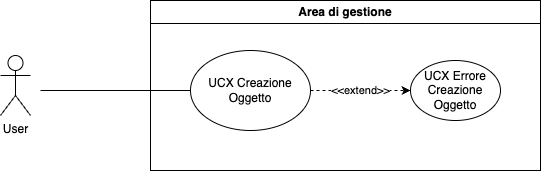
\includegraphics[width=0.8\textwidth]{UseCasesImages/ObjCr.png}
%\end{figure}
\large\textbf{} \\
\textbf{Attori:} User\\
\textbf{Pre-condizione:} Scaffallatura correttamente presente \\
\textbf{Post-condizione: } Visualizzazione dati scaffalatura\\
\textbf{Scenario Principale:}  L'utente sta navigando\textsuperscript{G} all'interno del magazzino e prova a selezionare una scaffalatura esistente. \\
\vspace{0.5cm}
